%----------------------------------------
% Preamble to set up the document
%----------------------------------------
\documentclass{article}

% set up packages (you shouldn't need to touch this)
\usepackage{graphicx}  % required to insert images
\usepackage{hyperref}  % for hyperlinks
\usepackage[svgnames]{xcolor}  % to change hyperlink colors
\colorlet{linkcolour}{DarkBlue}
\hypersetup{colorlinks=true, linkcolor=linkcolour, citecolor=linkcolour, urlcolor=linkcolour,}
\graphicspath{ {figures/} }
\usepackage{float}

% Margins
\topmargin=-0.45in
\evensidemargin=0in
\oddsidemargin=0in
\textwidth=6.5in
\textheight=9.0in
\headsep=0.25in

% use a sans serif font
\renewcommand{\familydefault}{\sfdefault}

%----------------------------------------
% Step 1: Edit the lecture title
%----------------------------------------
\title{
Lecture 4: Data manipulation and visualization in R \\  % Lecture title
Modeling Social Data, Spring 2019 \\   % Course title
Columbia University                    % School
}

%----------------------------------------
% Step 2: Edit your name and the date
%----------------------------------------
\author{Mia Fryer}                     % Scribe's name
\date{February 15, 2019}                % Lecture date

\begin{document}


\maketitle
\section{Overview}
\begin{itemize}
    \item Intro To R
        \begin{itemize}
            \item Why R?
            \item An Overview of the basics
        \end{itemize}
    \item tidyverse
        \begin{itemize}
            \item Overview
            \item dplyr
                \begin{itemize}
                     \item filter
                     \item arrange
                     \item select
                     \item mutate
                     \item group\_by
                     \item summerize
                     \item \%\textgreater\% (Pipe)
                     \item gather
                     \item spread
            \end{itemize}
        \end{itemize}
    \item Data Visualization
        \begin{itemize}
            \item Why Visualize
            \item Methods of Visualization
            \item ggplot2
        \end{itemize}
\end{itemize}


\section{Intro to R}
\subsection{Why R?}

While R is by no means a perfect language, it happens to be a wonderful tool for data analysis. Once learned it facilitates the transfer of ideas from brain to computer screen with as little friction as is currently possible.

\begin{flushleft}
Some examples of how R can be a bit unruly are as follows
\end{flushleft}

\begin{itemize}
    \item There is not standard case convention so seeing camelCase, this.that, and snake case conventions mixed and matched is not uncommon.
    \item Dots (.) (mostly) don’t mean anything special
    \item \$ gets used in funny ways
    \item R is very flexible in nature, and does many things for you behind the scenes which can lead to unexpected results if not careful. 
\end{itemize}

\subsection{An Overview of the basics}

\begin{flushleft}
Where R shines its ability to go from raw data to results quickly and efficiently, allowing you to "ask more questions"
\end{flushleft}

\begin{figure}[H]
    \centering
    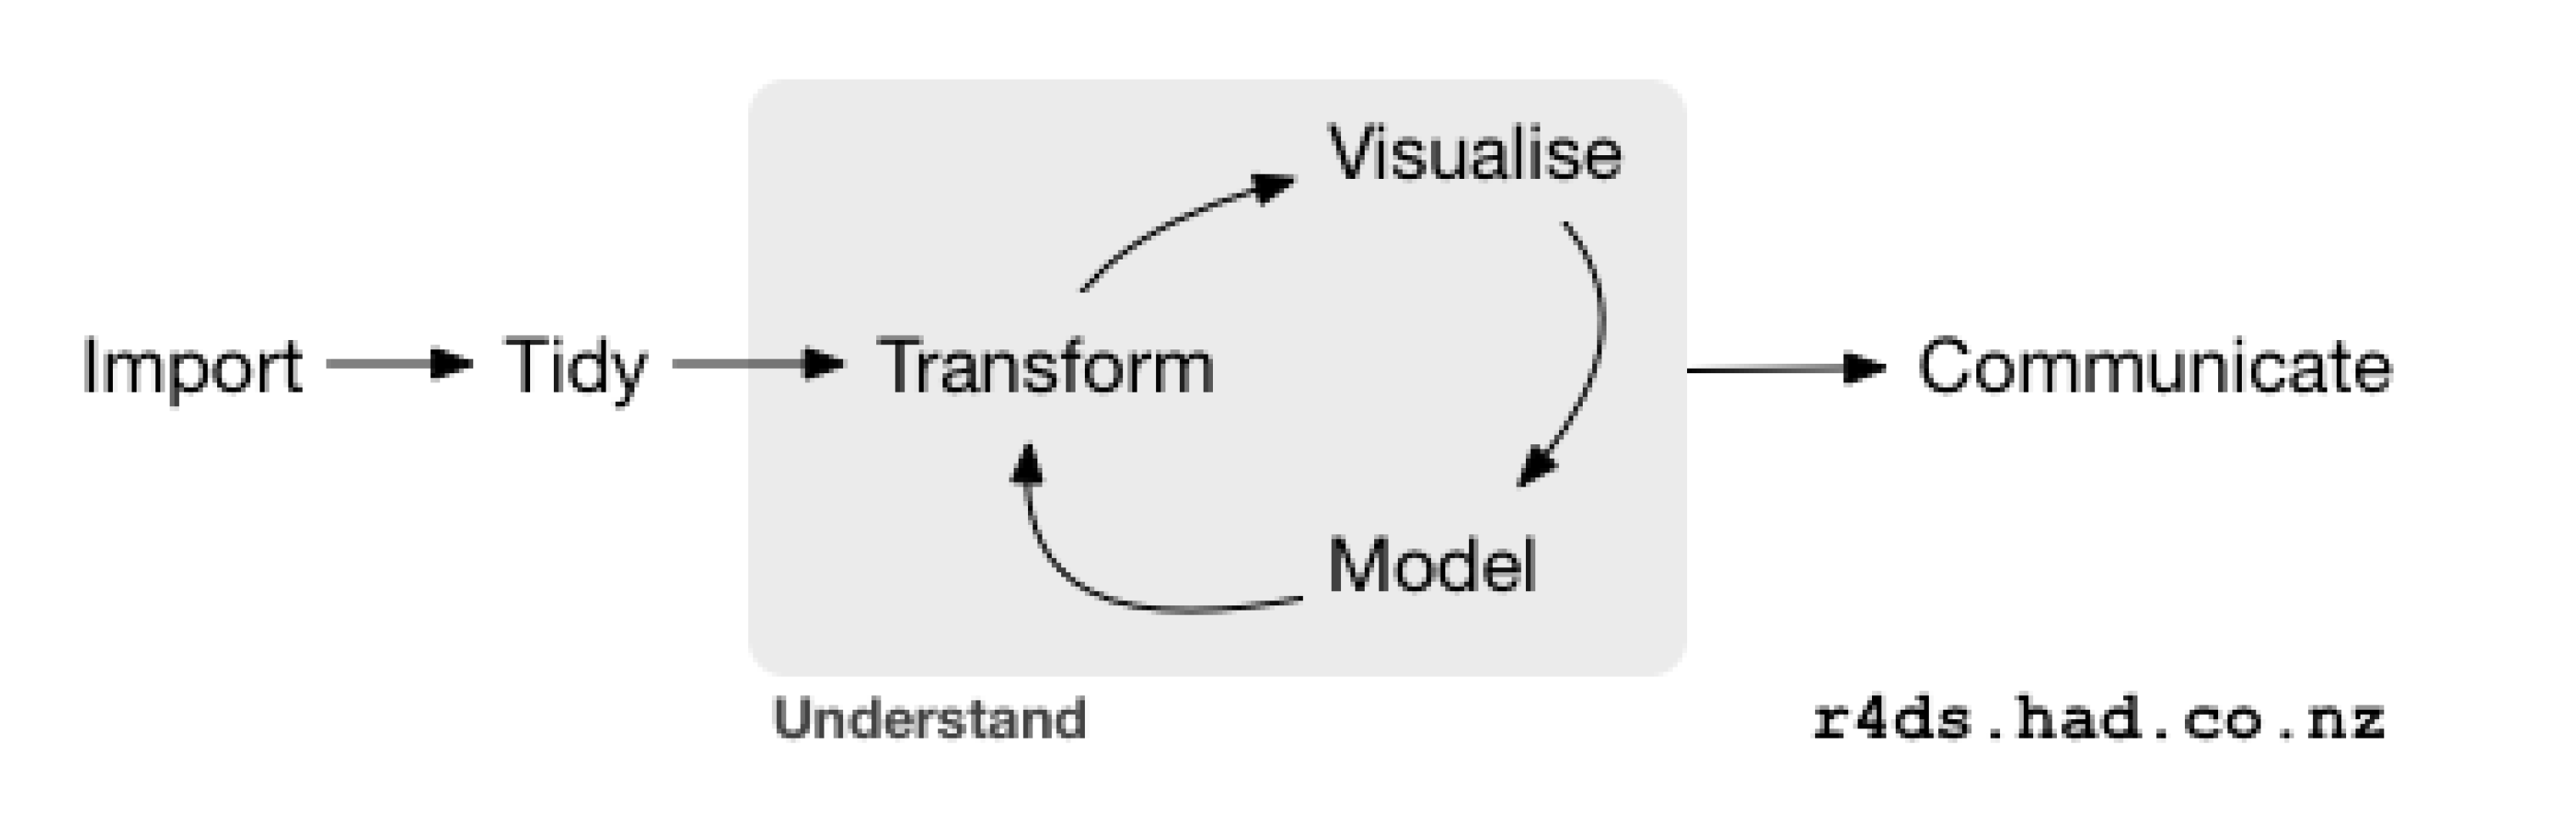
\includegraphics[width=.6\textwidth]{data_analysis_cycle.png}
    \caption{The data analysis cycle}
    \label{fig:data_analysis_cycle}
\end{figure}

\begin{flushleft}
In R there are basic data types which behave in different ways

\begin{itemize}
    \item int, double: for numbers
    \item character: for strings
    \item factor: for categorical variables (similart to struct or ENUM a factor is categorical variable where strings or values are categorized) 
\end{itemize}

As well as the type of individual data, the containers for this data have their own characteristics 

\begin{itemize}
    \item vector: for multiple values of the same type (~ array)
    \item list: for multiple values of diferent types (~ dictionary)
    \item data.frame: for tables of rectangular data of mixed types (~ matrix)
\end{itemize}

We'll mostly work with data frames, which themselves are lists of vectors

\end{flushleft}


\section{tidyverse}
\subsection{Overview}

\begin{flushleft}
tidyverse is the brain child of Hadley Wickham, and while he would most definitely scold us for giving him the credit for the creation and upkeep of tiderverse, his work on this package and many others has helped propel the work of data scientists around the world.
\end{flushleft}

\begin{flushleft}
The tidyverse itself is a collection of packages including
\begin{itemize}
    \item dplyr for split / apply / combine type counting
    \item ggplot2 for making plots
    \item tidyr for reshaping and “tidying” data
    \item readr for reading and writing files
\end{itemize}

\end{flushleft}

\begin{figure}[H]
    \centering
    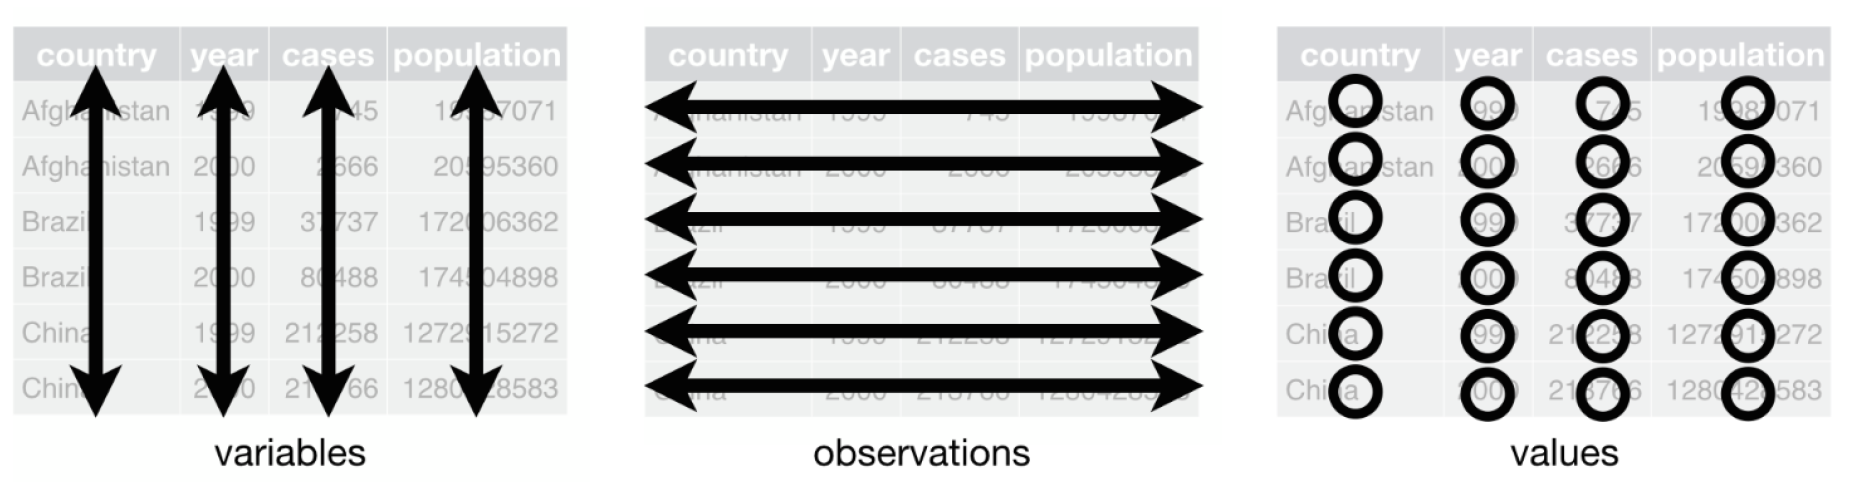
\includegraphics[width=.65\textwidth]{tidy_table.PNG}
    \caption{A representation of a "tidy table"}
    \label{fig:tidy_table}
\end{figure}

\begin{flushleft}

The core philosophy of tidyverse is that all data should be in a “tidy” table (As see in Figure 2) which means:
\begin{itemize}
    \item One variable per column
    \item One observation per row
    \item One measured value per cell
\end{itemize}
\end{flushleft}


\subsection{dplyr}

\begin{flushleft}
On the data manipulation side of "tidyverse" we have the library \textbf{dplyr}. The functions in \textbf{dpylr} we are going to go over today are as follows: filter, arrange, select, mutate, group\_by, summerize, \%\textgreater\% (Pipe), gather, spread
\end{flushleft}

\subsubsection{filter}
\begin{flushleft}
filter is a function which allows you to filter through a data frame with specific criteria. Utilizing the structure 
\textbf{filter(Data Frame, Criteria 1, Criteria 2, ...)}
\end{flushleft}

\begin{flushleft}
A example of how we can filter in the data set we are utilizing for our homework (citibike) is as follows
\end{flushleft}
\begin{center}
filter(trips, start\_station\_name == "Broadway \& E 14 St")
\end{center}

\begin{figure}[H]
    \centering
    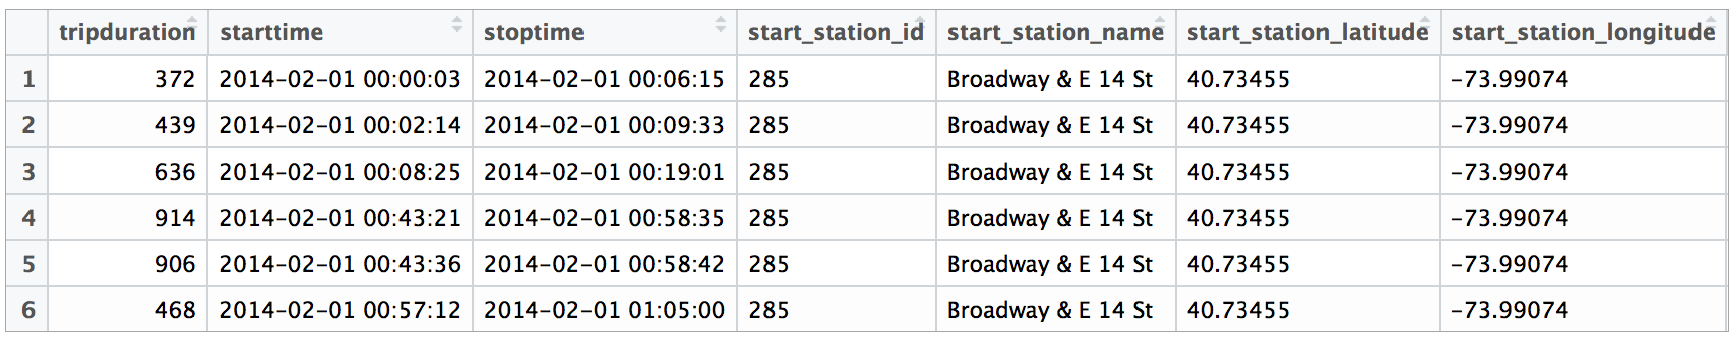
\includegraphics[width=.75\textwidth]{filter_trips_ex.png}
    \caption{Example: Trips Filtered for trips that start on Broadway}
    \label{fig:filter_trips_ex}
\end{figure}

\begin{flushleft}
\textbf{Whats weird about this?} if you've looked at the data set for homework one there is no object named start\_station\_name, intead start\_station\_name is a column. This means that the command filter is taking care of the scope for you, meaning you don't have to index to the specific column like you would in other languages. This is very convenient because it allows you to work naturally.
\end{flushleft}

\subsubsection{arrange}
\begin{flushleft}
The function arrange is a nifty function that allows you to sort columns in your data set. following the structure of \textbf{arrange(Data Frame, column to sort, ...)} adding of course any sort modifiers you might want to include
\end{flushleft}


\subsubsection{select}
\begin{flushleft}
The select function allows you to choose which rows you want to display or pass on to another function (more on that later). The format of the select function is as follows \textbf{select(Data Frame, Column1, Column 2, ...)} Lets look at an example.
\end{flushleft}

\begin{center}
select(trips, starttime, stoptime,start\_station\_name, end\_station\_name)
\end{center}

\begin{figure}[H]
    \centering
    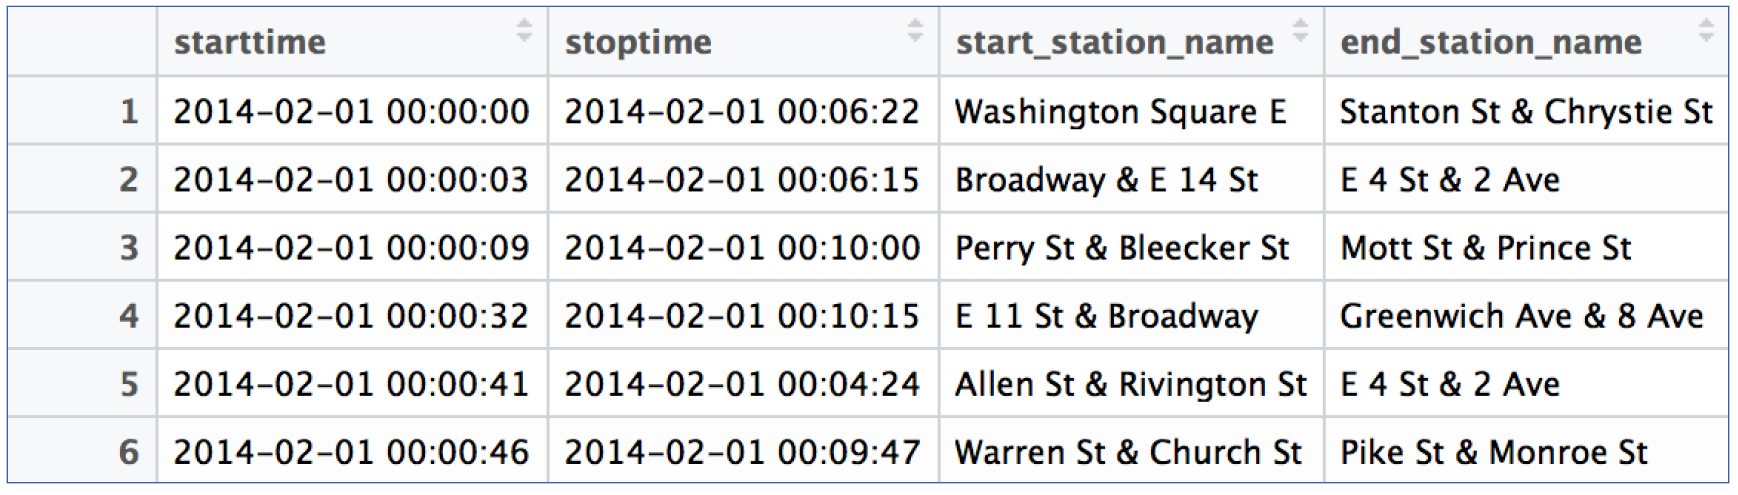
\includegraphics[width=.75\textwidth]{select_trips_ex.PNG}
    \caption{Example: Start Time, Stop Time, Start Station, and End Station are the columns displayed}
    \label{fig:select_trips_ex}
\end{figure}


\subsubsection{mutate}
\begin{flushleft}
The mutate function allows you to create new data columns by doing an operation on one or more data columns. The resulting calculation will be put into a new column which you can either name or have auto named. 
\end{flushleft}

\begin{center}
mutate(trips, time\_in\_min = tripduration \textbackslash 60)
\end{center}

\begin{figure}[H]
    \centering
    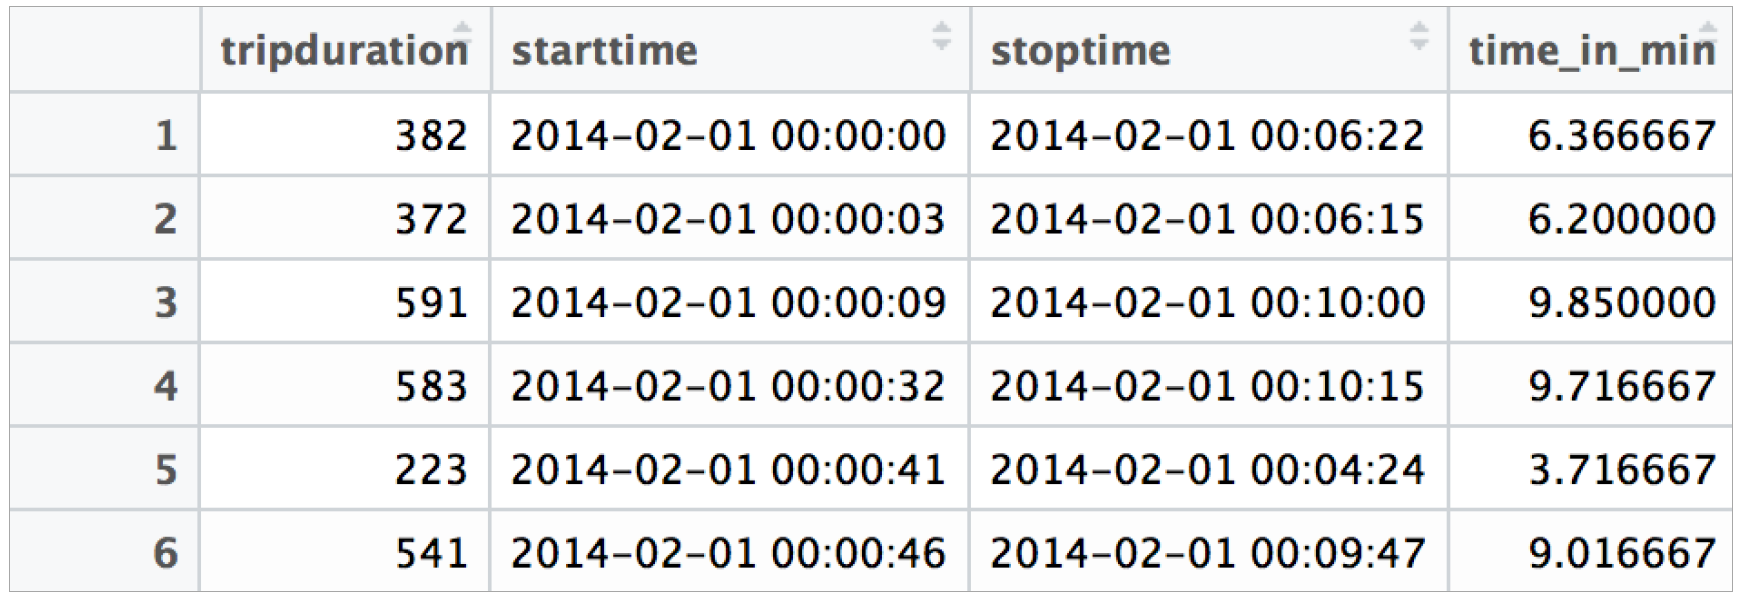
\includegraphics[width=.75\textwidth]{mutate_trips_ex.png}
    \caption{Example: setting a new column time in minutes equal to the trip duration divided by 60 (since the trip duration is in seconds)}
    \label{fig:mutate_trips_ex}
\end{figure}


\subsubsection{group\_by}
\begin{flushleft}
The group\_by command allows you to keep track of groups within a data frame. This is useful especially when combined with the summarize function which will be covered shortly. An example of grouping can be seen below
\end{flushleft}

\begin{center}
trips\_by\_gender <- group\_by(trips, gender)
\end{center}    

\begin{figure}[H]
    \centering
    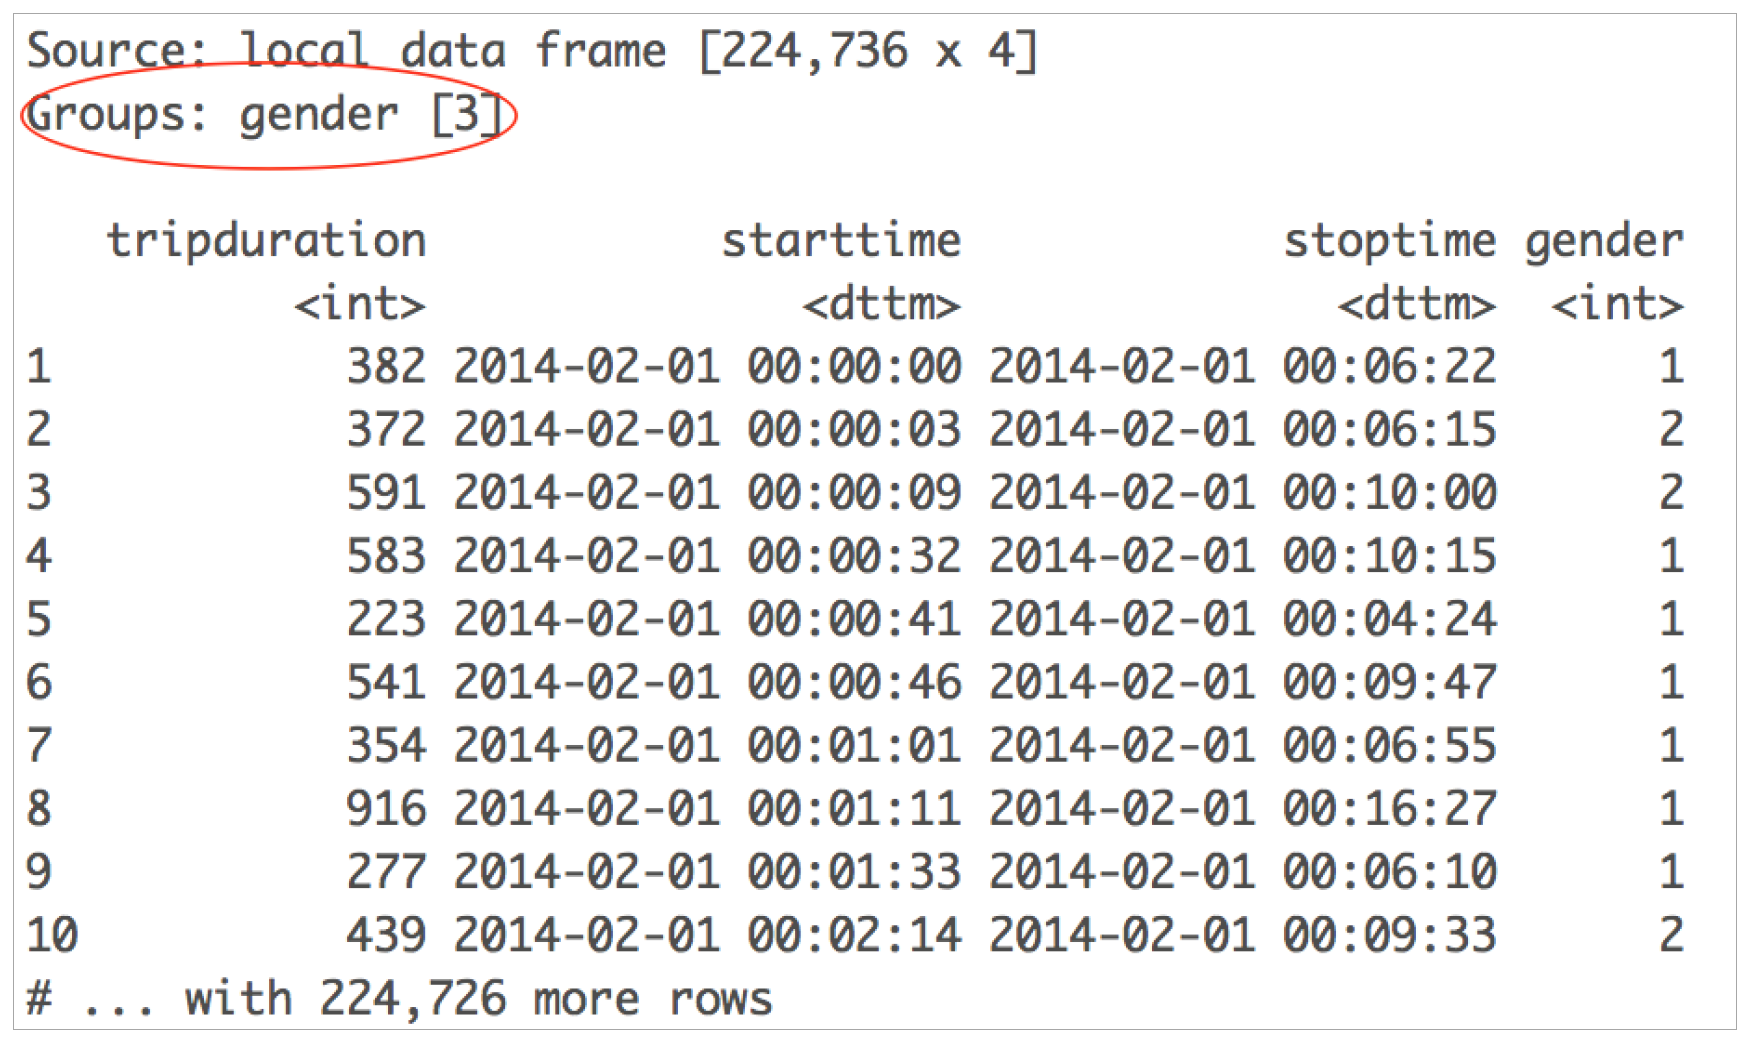
\includegraphics[width=.75\textwidth]{group_by_gender.png}
    \caption{Example: In this example, we are grouping by gender and storing the values in a new data frame called trips\_by\_gender noticed the red circle. We have three groups 1 = male, 2 = female, 0 = unknown}
    \label{fig:group_by_gender}
\end{figure}

\begin{flushleft}
\textbf{A word of caution} when using the group\_by function, after you're done with it you will want to un-group. This is due to the fact that when you group you're adding on a separate index which holds what "groups" are in the data set. So when you run summarize, it will take these groups and give you statistics for each one. However if you are done analyzing those groups, it could make for some problematic results when trying to get statistics for other matters of interest. So in short after you're done using a group for analysis \textbf{Always un-group}
\end{flushleft}

\subsubsection{group\_by + summarize}
\begin{flushleft}
The summarize command allows input queries such as mean and standard deviation and computes these queries for the data you input into it. This can be truly powerful when used in conjunction with the group\_by function as you can then look for specific statistics for specific groups you are interested in. 
See example below
\end{flushleft}

\begin{center}
summarize(trips\_by\_gender, count = n(), mean\_duration = mean(tripduration) \textbackslash 60, sd\_duration = sd(tripduration) \textbackslash 60)
\end{center}    

\begin{figure}[H]
    \centering
    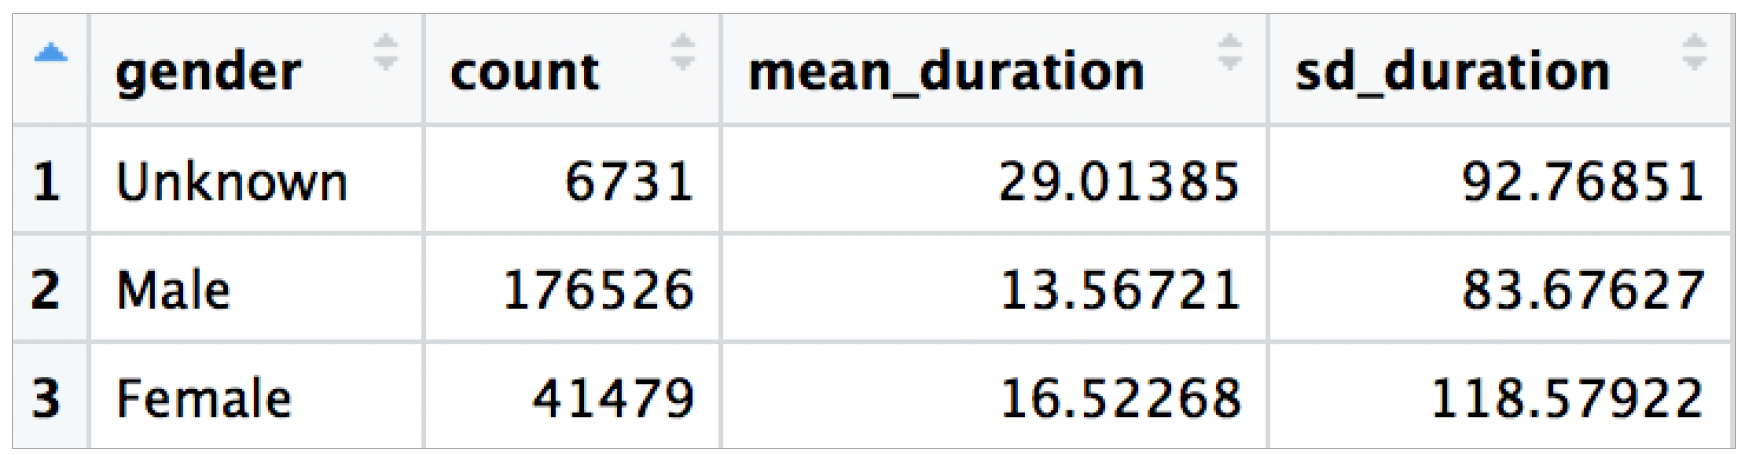
\includegraphics[width=.75\textwidth]{group_and_summarize.png}
    \caption{Example: Here we are looking for the count, mean, and standard deviation of trip duration by gender }
    \label{fig:group_and_summarize}
\end{figure}


\subsubsection{gather}
\begin{flushleft}
Using the gather command allows you too merge data sets in a way that combines columns. This might be useful in different situations where a transformation like this would help with the analysis of data. For our example below we wanted to see the sequential happenings of each trip instead of just when each trip starts and stops. This might help us calculate something like how many bikes are on the road at a given time. 
\end{flushleft}

\begin{flushleft}
Lets take the example of calculating how many bikes are on the road at a given time.
\end{flushleft}

\begin{center}
trips \%\textgreater\% gather("variable", "value", starttime, stoptime) \%\textgreater\% arrange(value) \%\textgreater\% mutate(delta = ifelse(variable == "starttime", 1, -1))
\end{center}    

\begin{figure}[H]
    \centering
    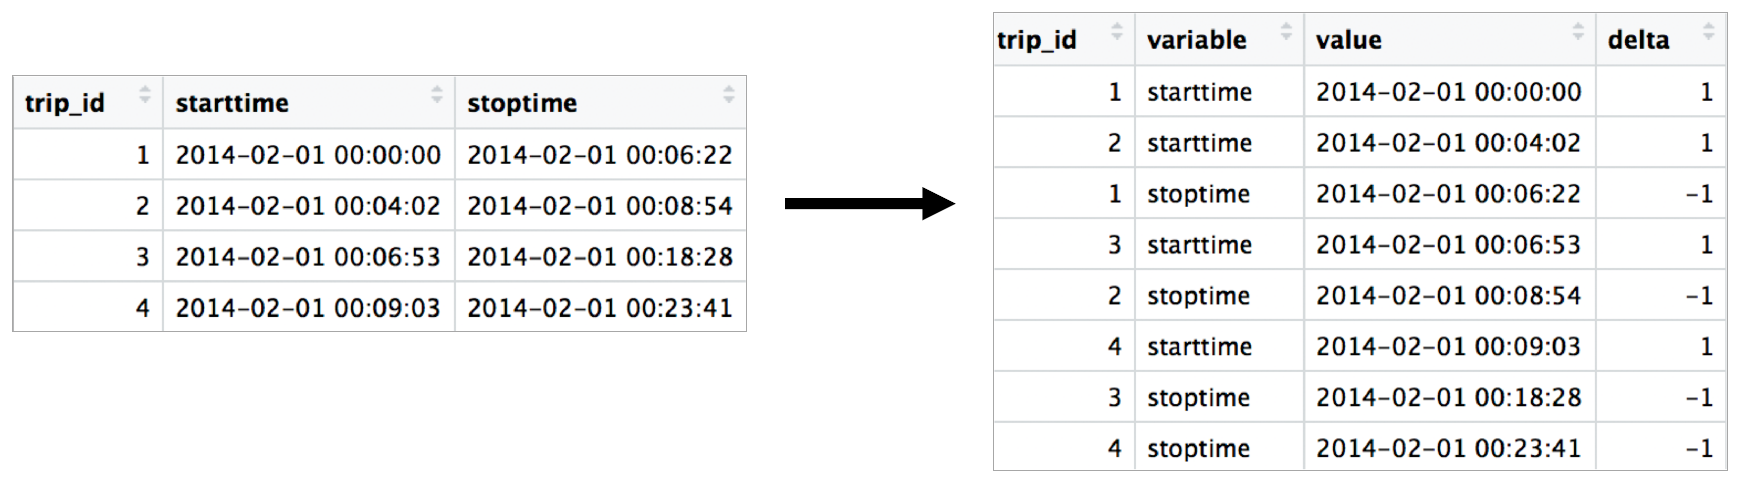
\includegraphics[width=.75\textwidth]{gather_ex.png}
    \caption{Example: By "gathering" the stop and start time in one column we can see the order of sequential events, by arranging these times it allows us to calculate how many bikes are on the road via the mutate function}
    \label{fig:gather_ex}
\end{figure}


\subsubsection{spread}
\begin{flushleft}
The spread function operates much like the gather function, but in reverse. Taking groups of data and making them separate columns. Looking at figure \ref{fig:gather_ex} the spread(variable, value) command would revert the columns on the right to the columns on the left.
\end{flushleft}


\section{Data Visualization}
\subsection{Why Visualize}

\begin{flushleft}
Data visualization serves two main purposes. First it allows you to see data and get a better overall view of what is going on. Second it allows us to communicate data to others in the most time effective way possible. 
\end{flushleft}

\begin{flushleft}
A great example of why data visualization is important can be seen in Anscombe’s quartet. As the name quartet implies, it is 4 data sets that share the same mean, variance, linear regression line, as well as other statistical measures as seen in the figure below.
\end{flushleft}

\begin{figure}[H]
    \centering
    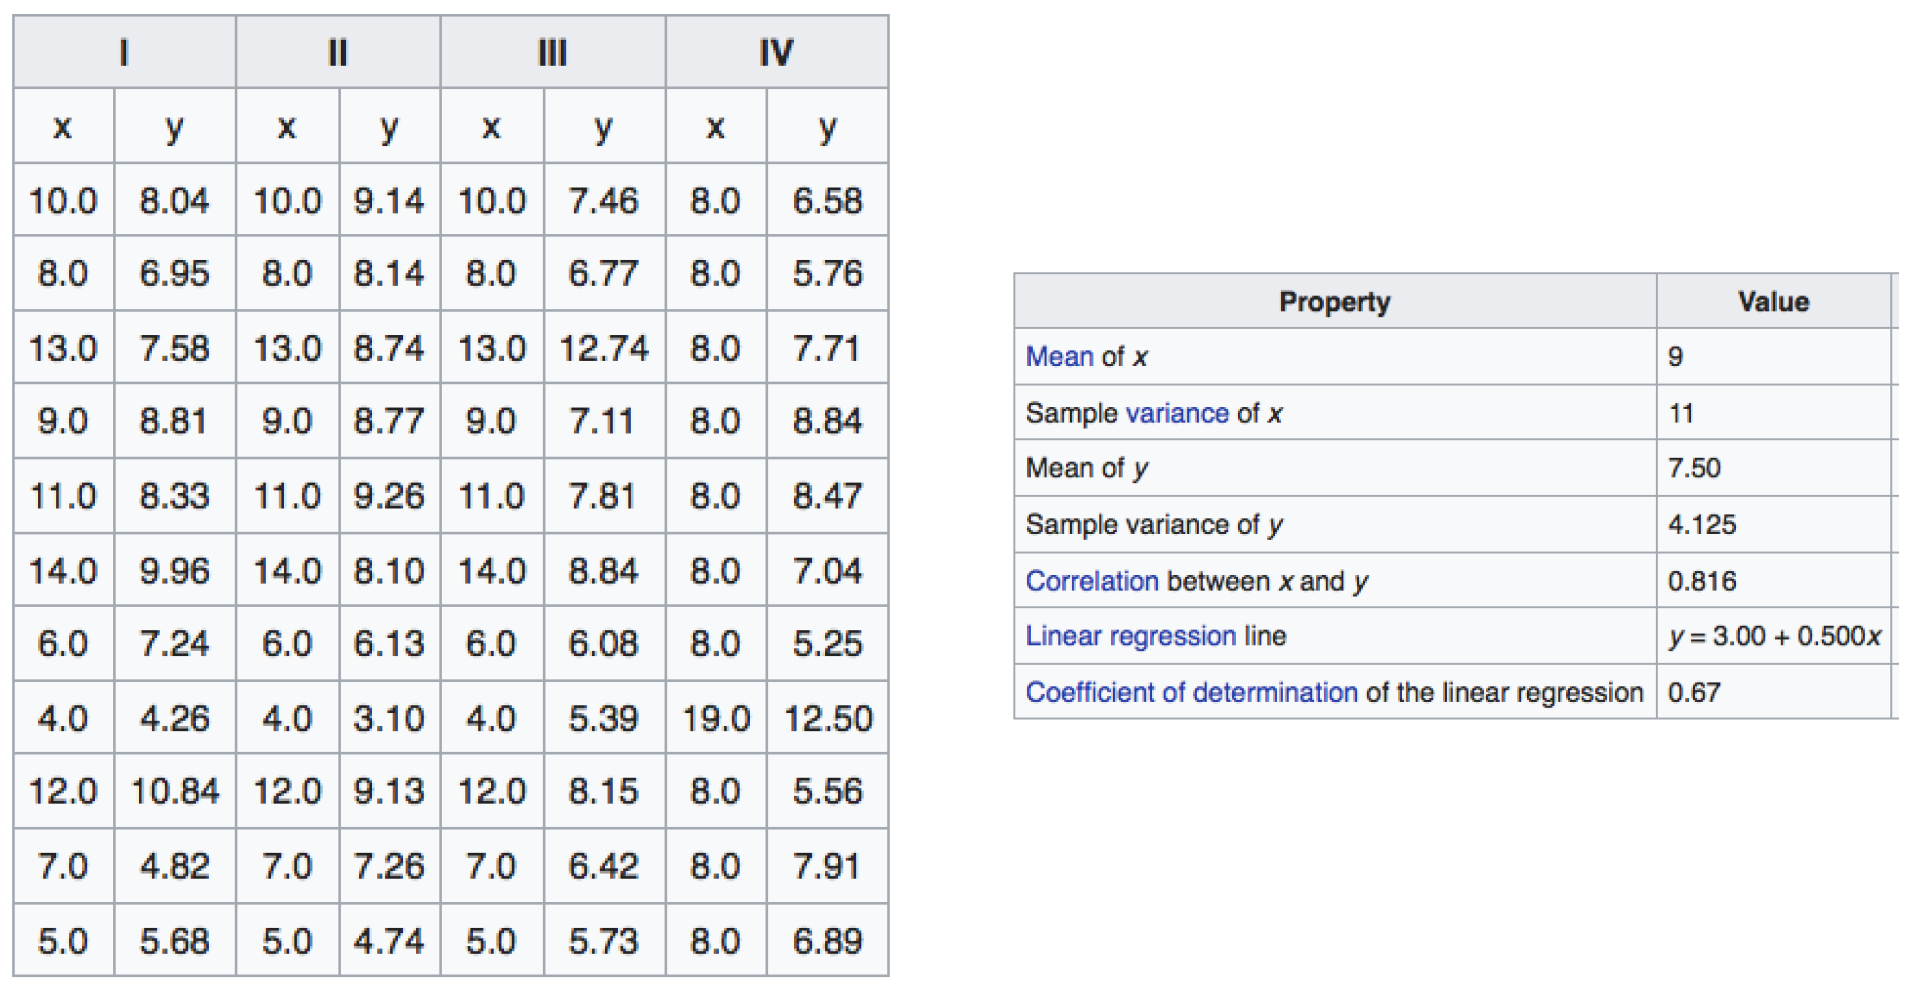
\includegraphics[width=.75\textwidth]{Anscombes_quartet.png}
    \caption{Example: Anscombe's quartet}
    \label{fig:Anscombes}
\end{figure}

\begin{flushleft}
When you look at each of these different data sets plotted out however, the story looks much different.
\end{flushleft}

\begin{figure}[H]
    \centering
    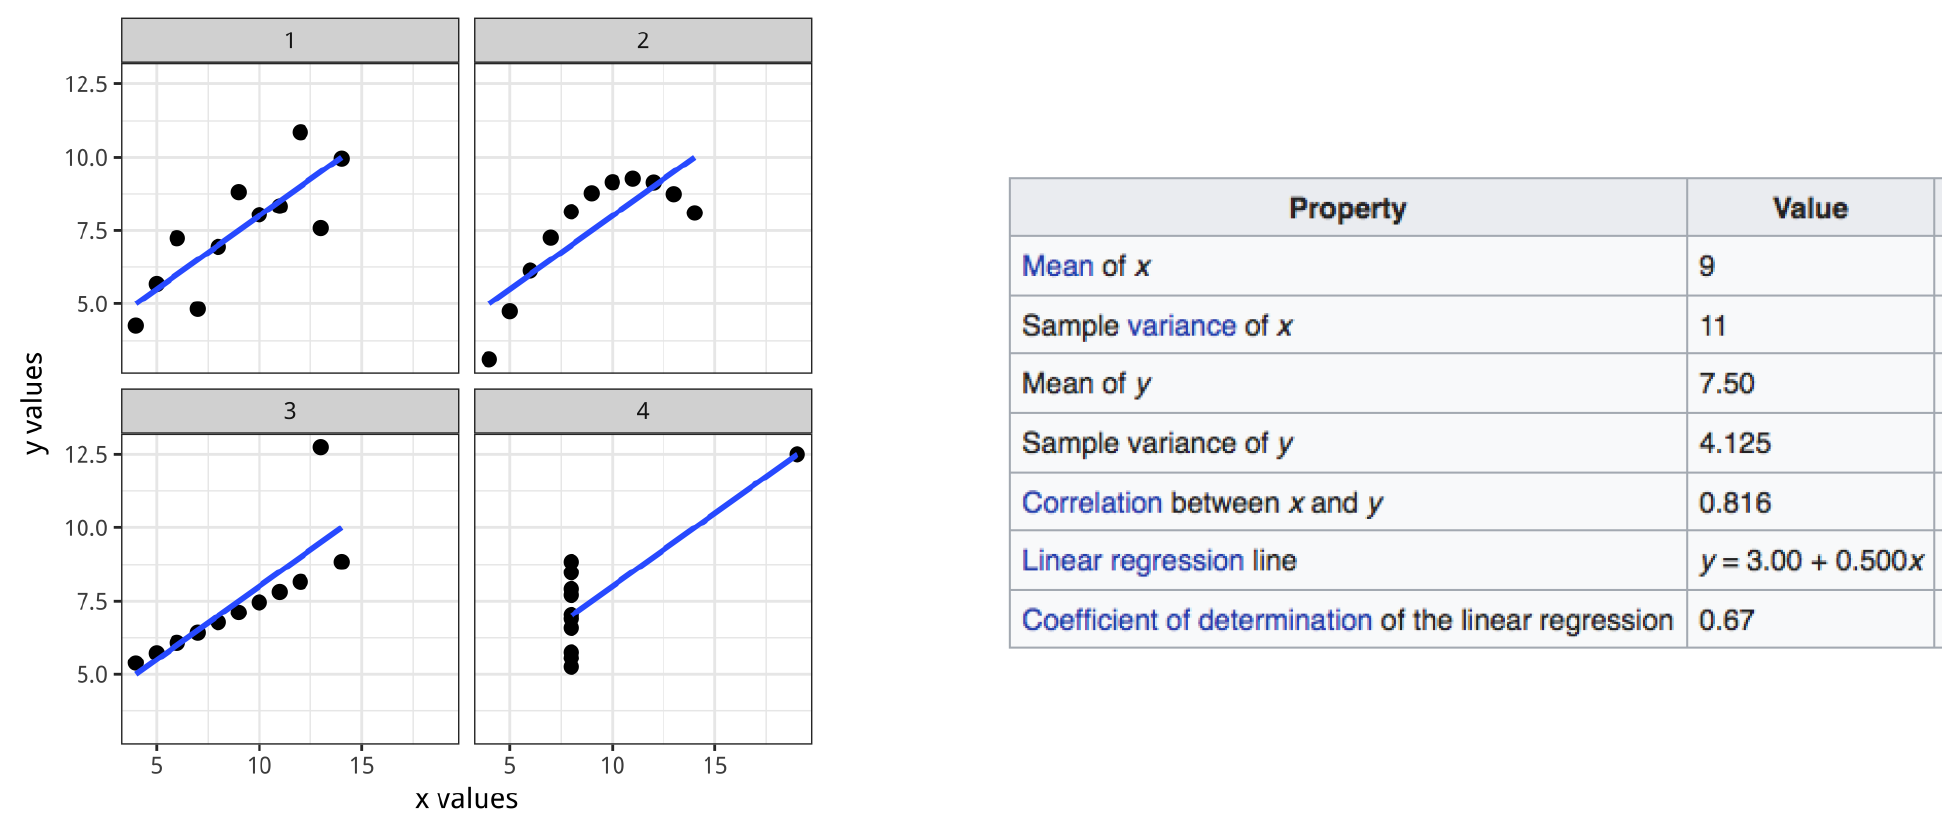
\includegraphics[width=.75\textwidth]{Anscombes_quartet_plotted.png}
    \caption{Example: Anscombe's quartet plotted}
    \label{fig:Anscombes_plotted}
\end{figure}

\subsection{Methods of Visualization}

\begin{flushleft}
As demonstrated in figure \ref{fig:Anscombes_plotted} plotting out data can reveal traits more quickly than reading of some statistical analysis of the data. However when it comes to generating information graphics for others to consume what is the best method of displaying said data?
\end{flushleft}
\begin{flushleft}
Obviously the answer to that question is a solid "It depends" but instead of trying to reinvent the wheel lets take a look at some of the research that has been done on the topic starting with a paper by \textbf{Jock Mackinlay} back in 1986
\end{flushleft}
\begin{flushleft}
In his paper entitled \textit{Automating the Design of Graphical Presentations of Relational Information} he espoused some basic principles of a good plot
    \begin{itemize}
        \item Good plots should express the facts effectively as possible
        \item “Tell the truth and nothing but the truth”
        \item Use encodings that people can easily decode
        \item Make a clear and concise point
        \item Have a one sentence take-away
    \end{itemize}
\end{flushleft}
\begin{flushleft}
He also broke down how we as humans perceive data, in terms of how accurately we can decipher different representations.
\end{flushleft}
\begin{figure}[H]
    \centering
    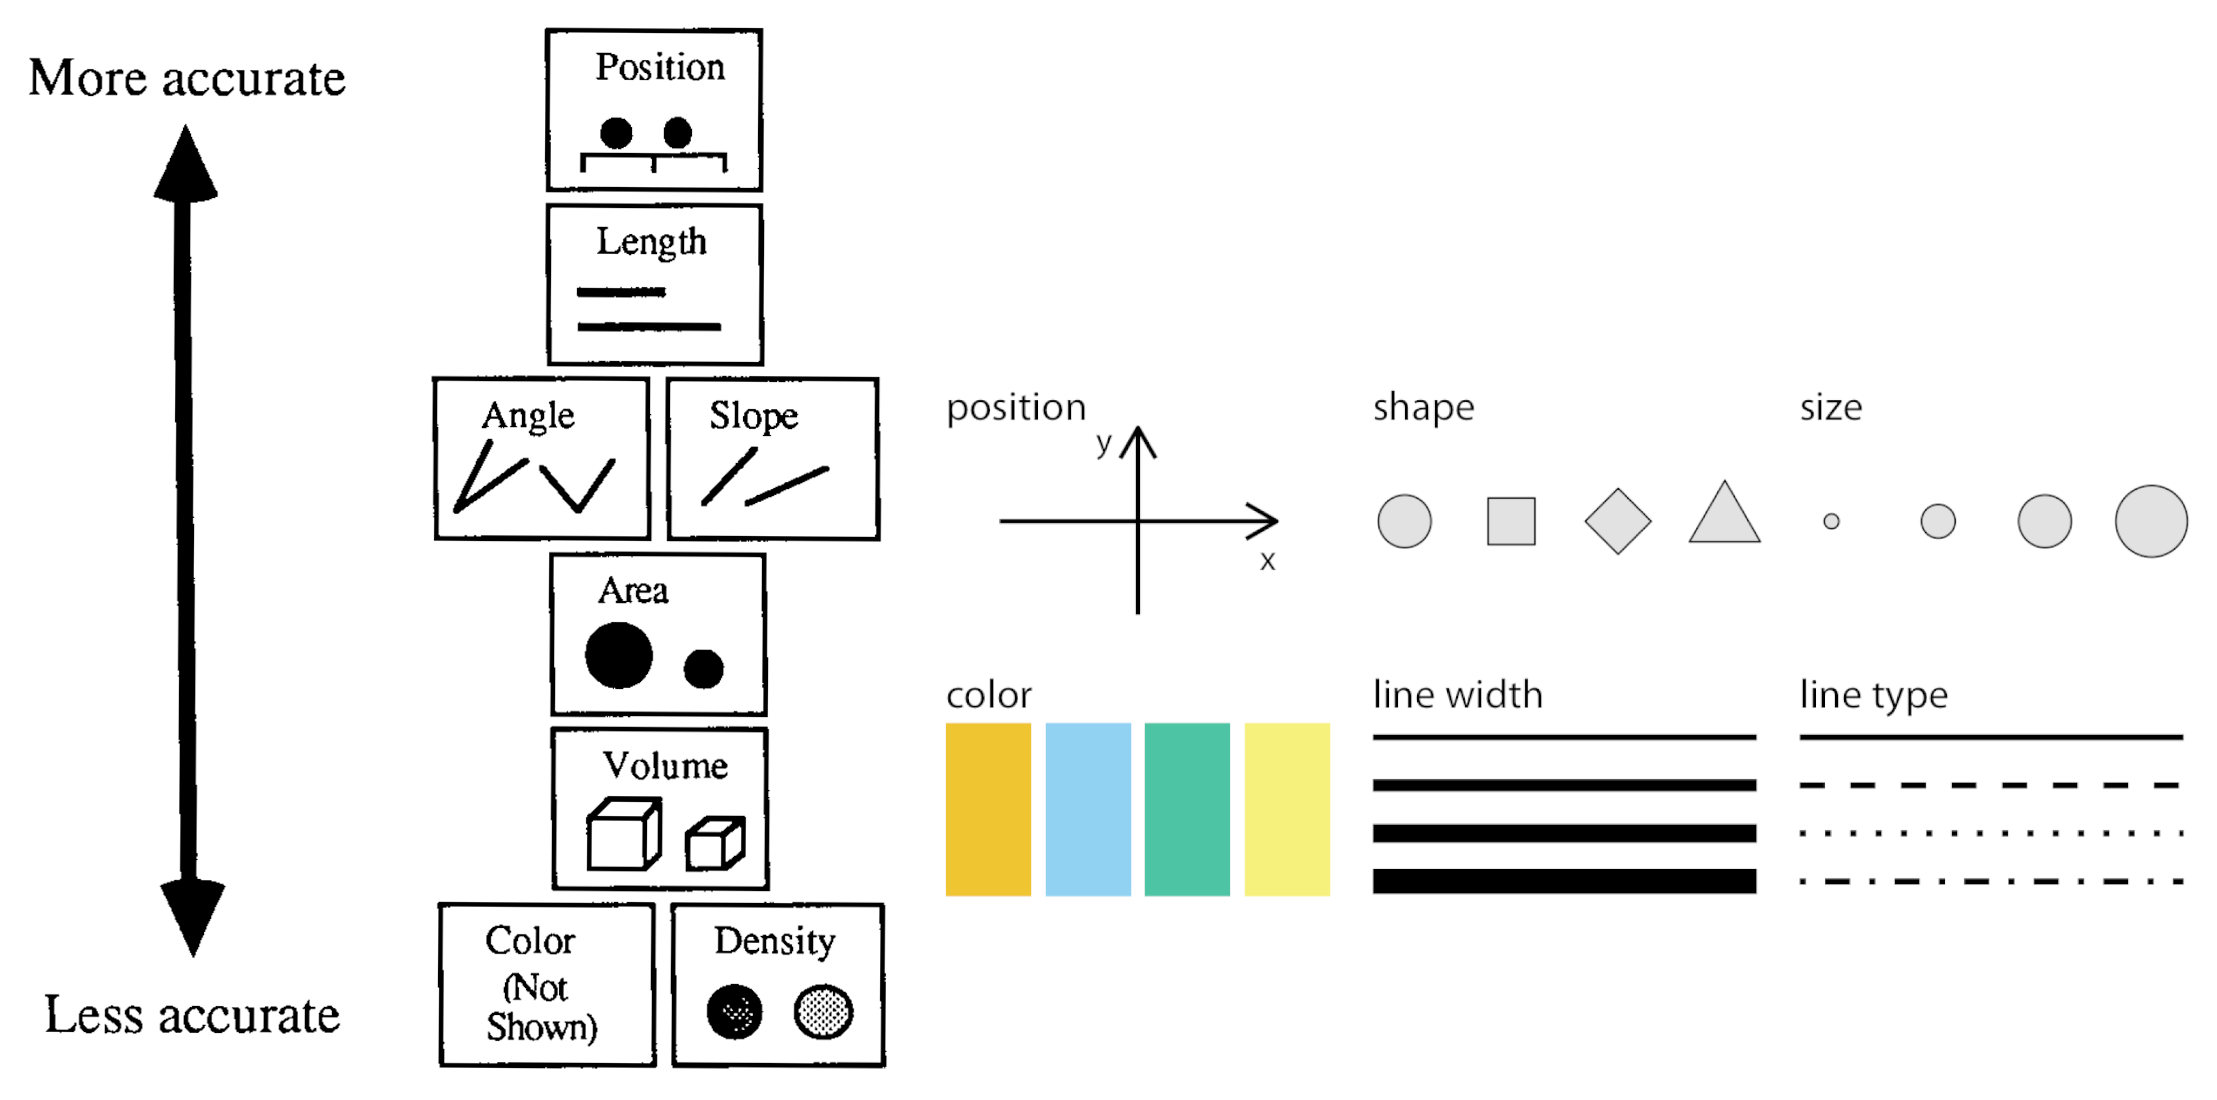
\includegraphics[width=.55\textwidth]{data_representation.png}
    \caption{Example: According toe Mackinlay, the arrow on the left indicates from easiest to understand on top to hardest to understand on bottom how accurate humans are at deciphering information from graphical representation}
    \label{fig:data_representation}
\end{figure}
\begin{flushleft}
Mackinlay further delved into the human readability of plots and data as he looked at the strokes for different data types. where Quantitative: numerical values in a range (e.g., height) Ordinal: categories with natural ordering (e.g., day of week) Nominal: categories with no natural ordering (e.g., gender) this can be seen in both figure \ref{fig:data_types_1} and figure \ref{fig:data_types_2}
\end{flushleft}
\begin{figure}[H]
    \centering
    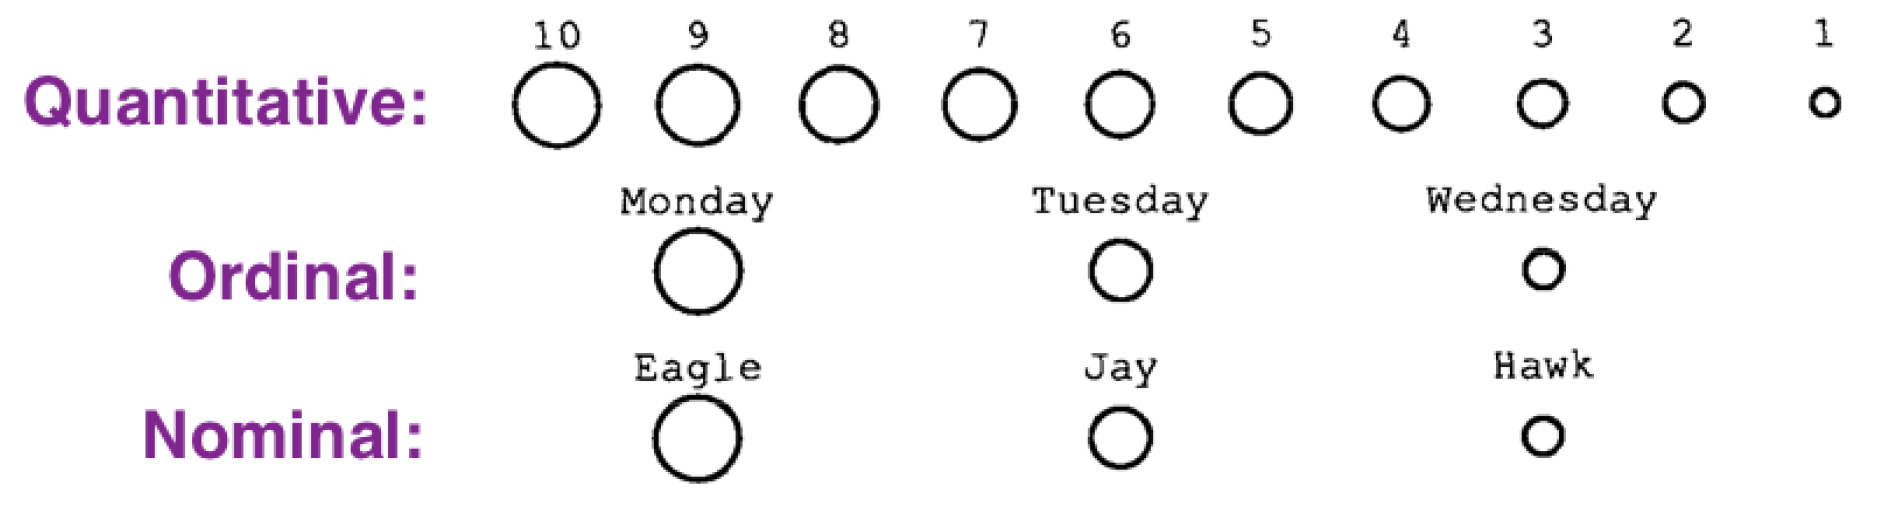
\includegraphics[width=.75\textwidth]{data_types_1.png}
    \caption{Analysis of the area task. The top case shoes that area is moderately effective for encoding quantitative information. The middle case shoes that is it possible to encode ordinal information as long as the step size between areas is large enough so that the values are not confused. the bottom case shows that it is possible to encode nominal information, but people may perceive an ordinal meaning.}
    \label{fig:data_types_1}
\end{figure}
\begin{figure}[H]
    \centering
    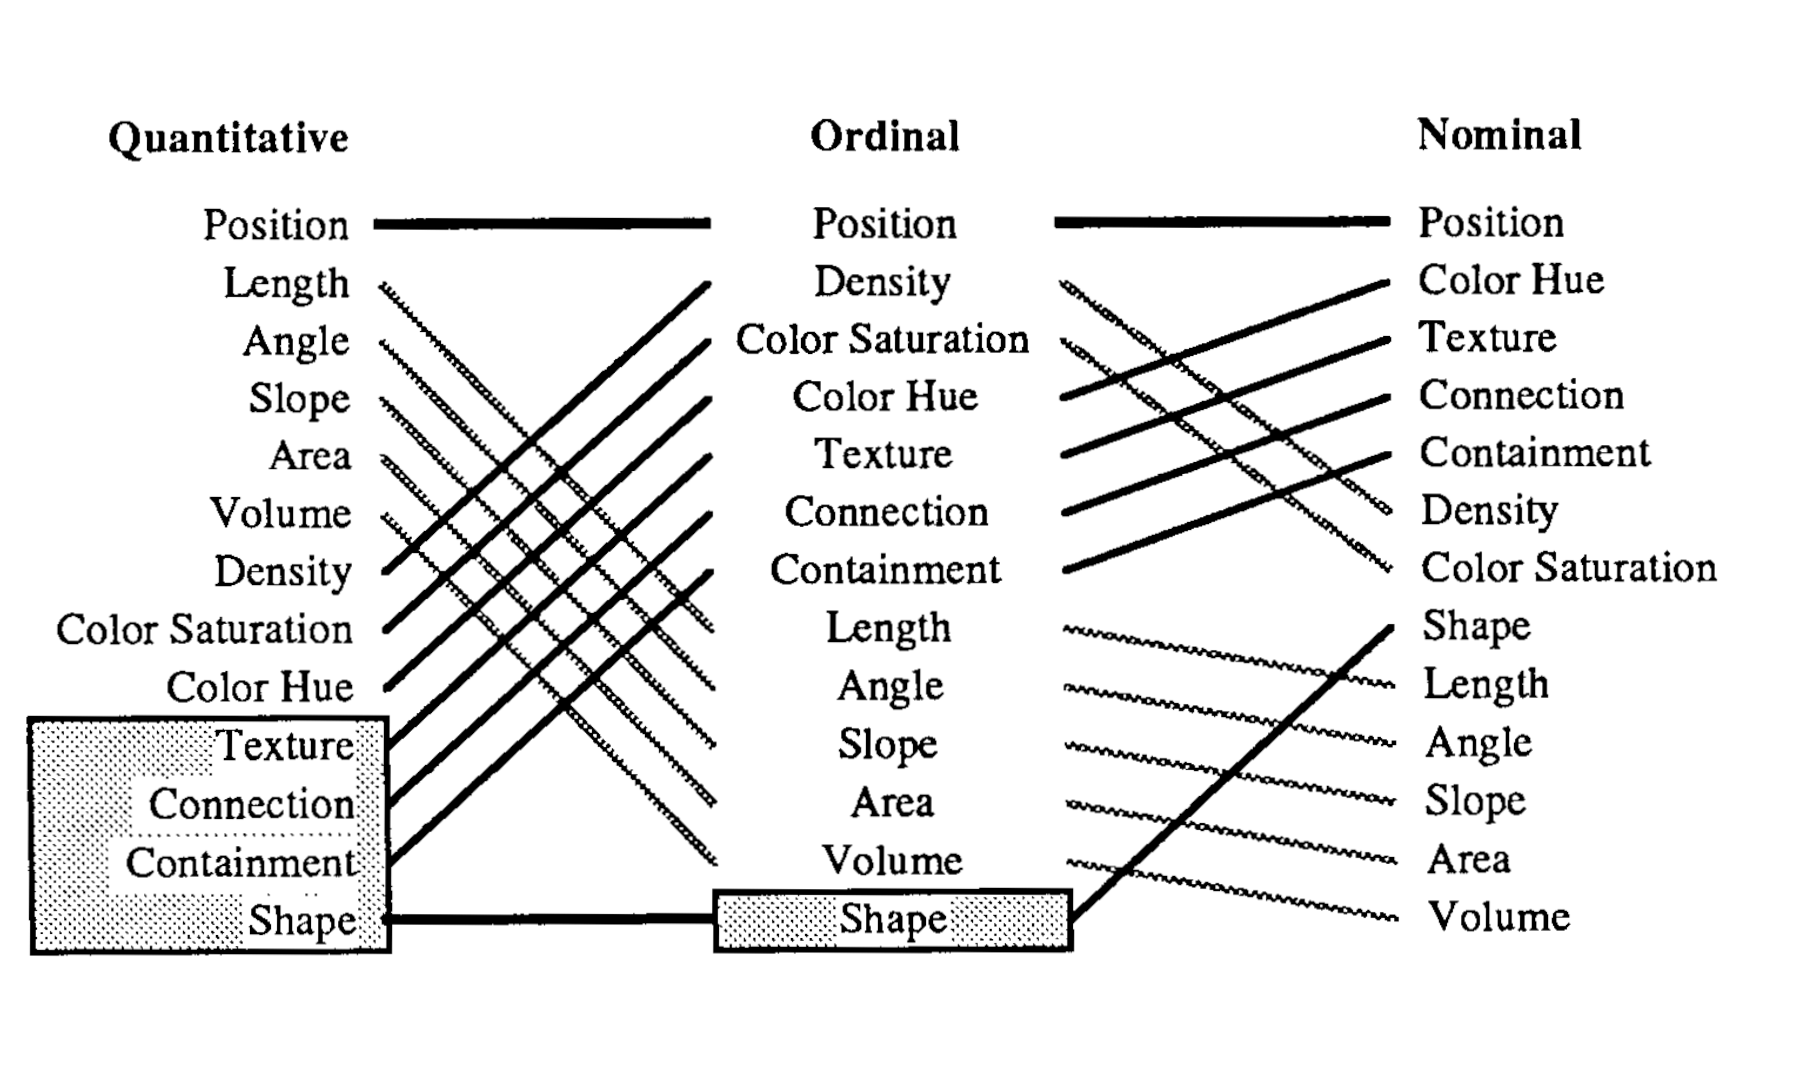
\includegraphics[width=.75\textwidth]{data_types_2.png}
    \caption{Ranking of perceptual tasks. The task shown in the gray boxes are not relevant to these types of data.}
    \label{fig:data_types_2}
\end{figure}


\subsection{ggplot2}
\begin{flushleft}
In the actual implementation of data visualization in R we are going to be using a package called ggplot2. 
\end{flushleft}
\begin{flushleft}
First off lets take a look at the grammer structure of how to write ggplot2 code.
\end{flushleft}
\begin{figure}[H]
    \centering
    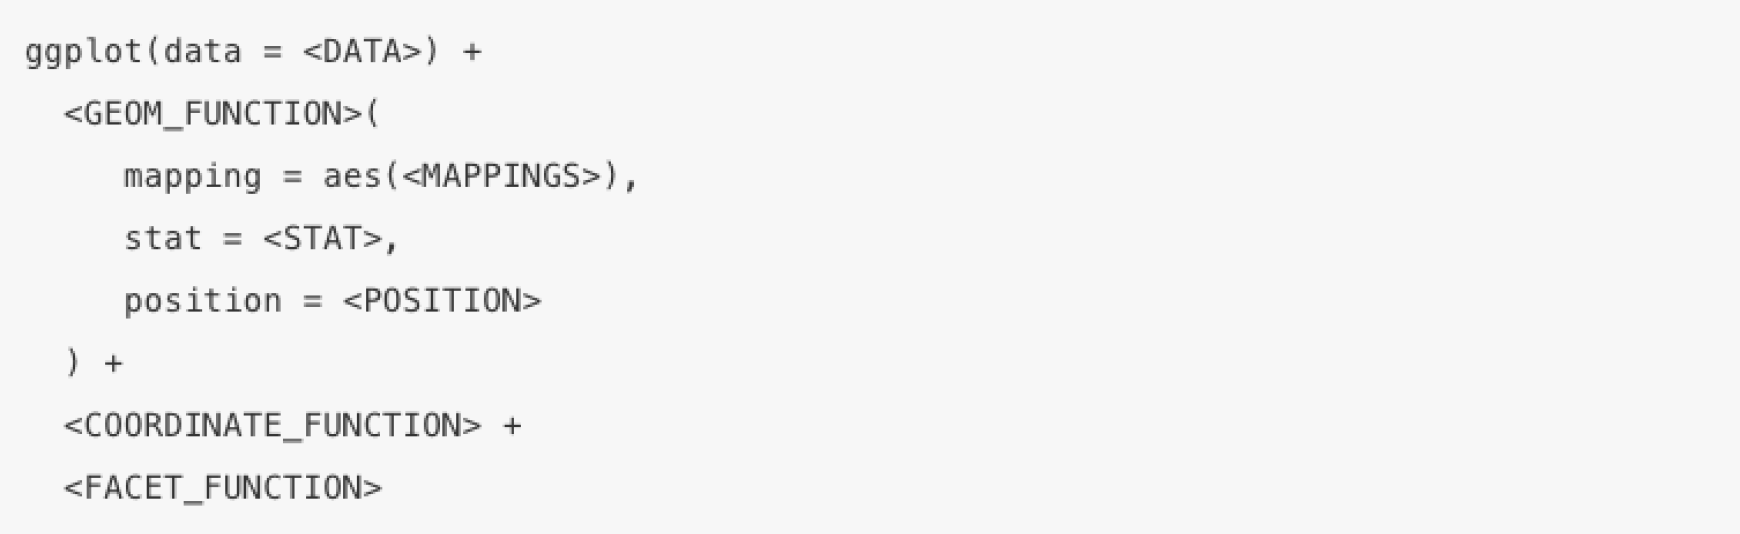
\includegraphics[width=.75\textwidth]{ggplot2_grammar.png}
    \caption{An overview of the grammatical structure of how to program a ggplot visualization}
    \label{fig:ggplot2_grammar}
\end{figure}
\begin{flushleft}
As with any type of work, its good to maintain a consistent work flow, in figure \ref{fig:ggplot_workflow} below is a good work flow to follow when using ggplot 
\end{flushleft}
\begin{figure}[H]
    \centering
    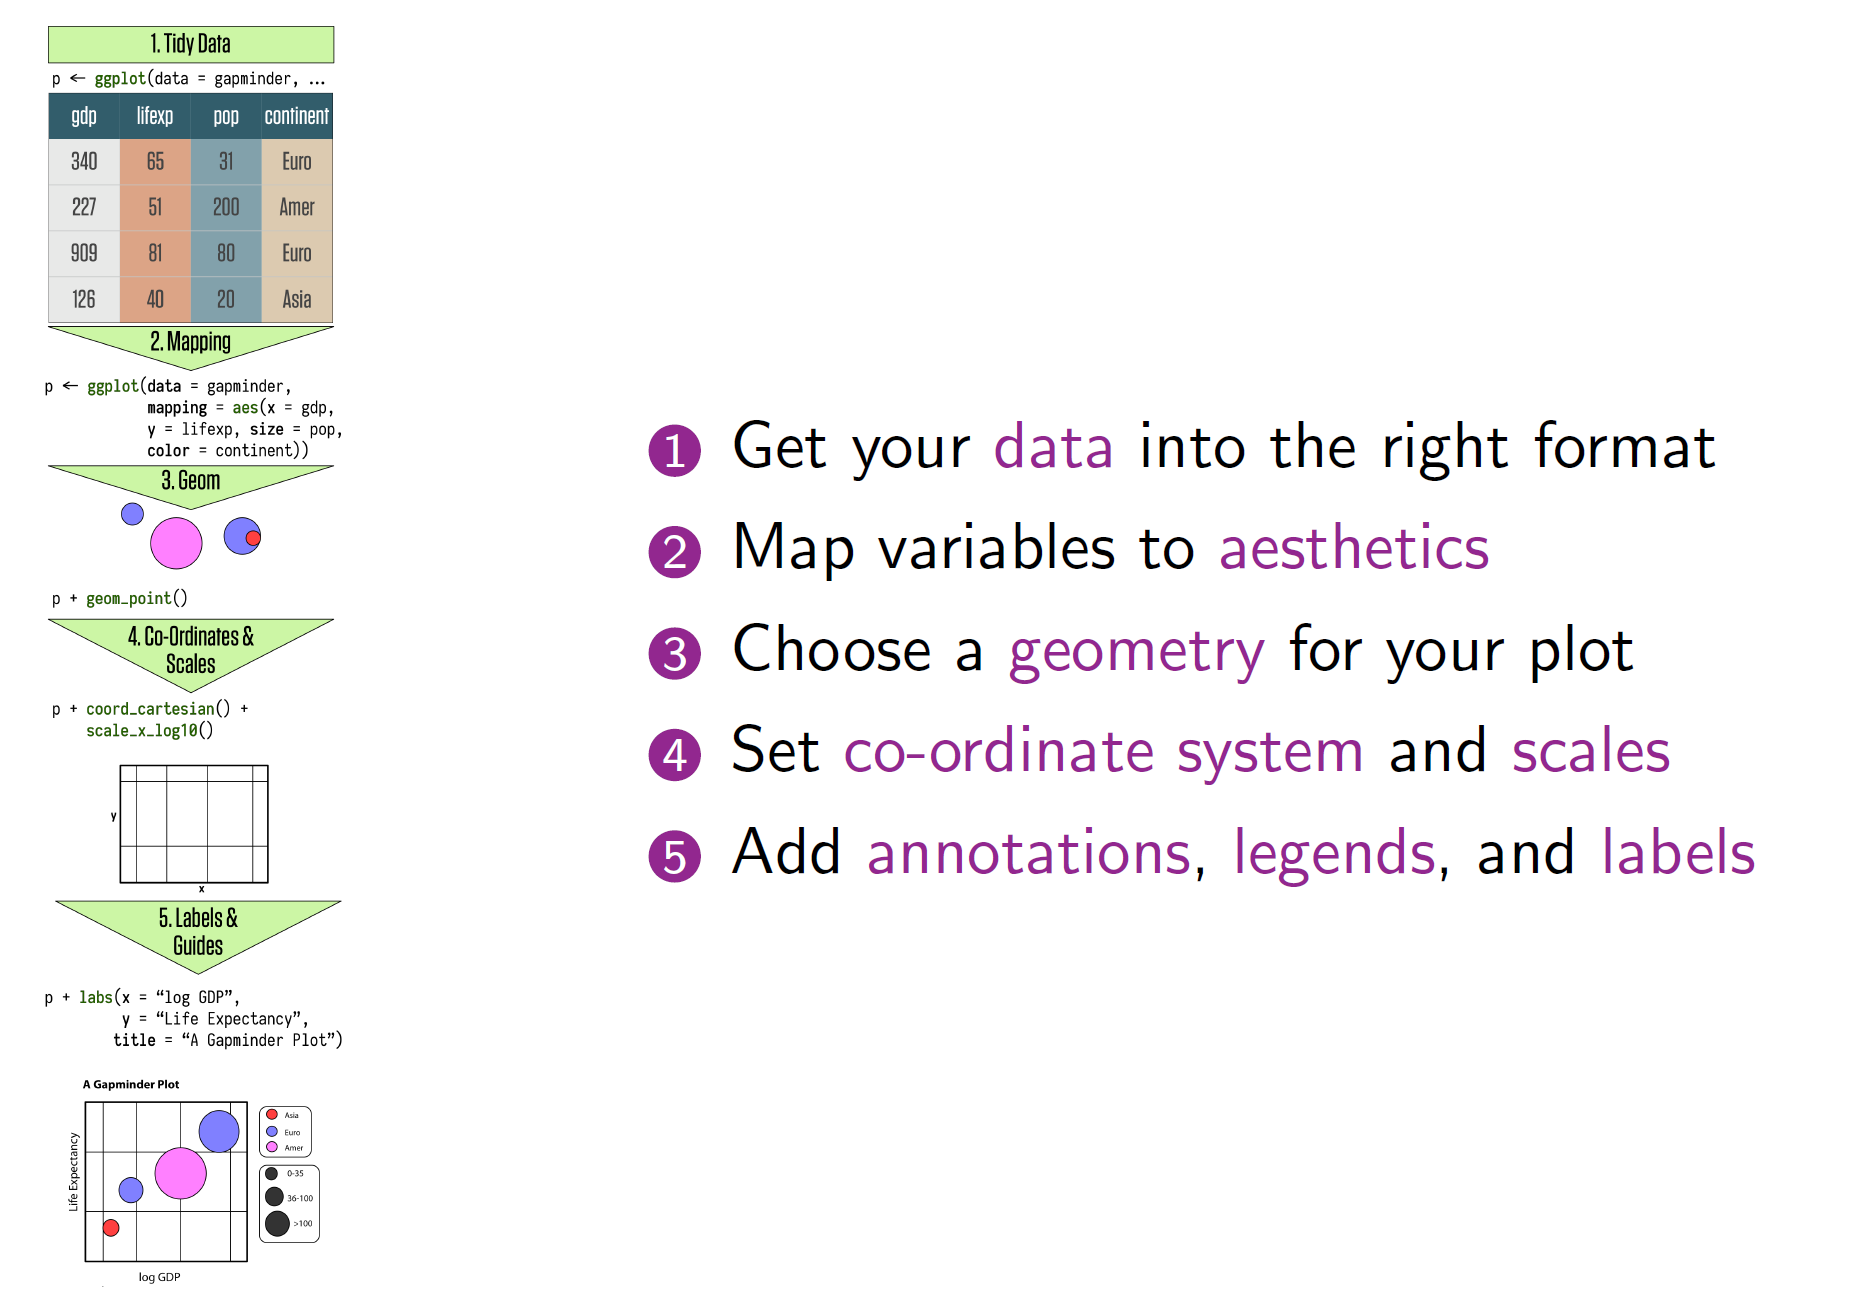
\includegraphics[width=.75\textwidth]{ggplot_workflow.png}
    \caption{ggplot work flow}
    \label{fig:ggplot_workflow}
\end{figure}
\begin{flushleft}
Finally lest dive into an example of how to use ggplot to plot the health and wealth of countries over time. 
\end{flushleft}
\begin{figure}[H]
    \centering
    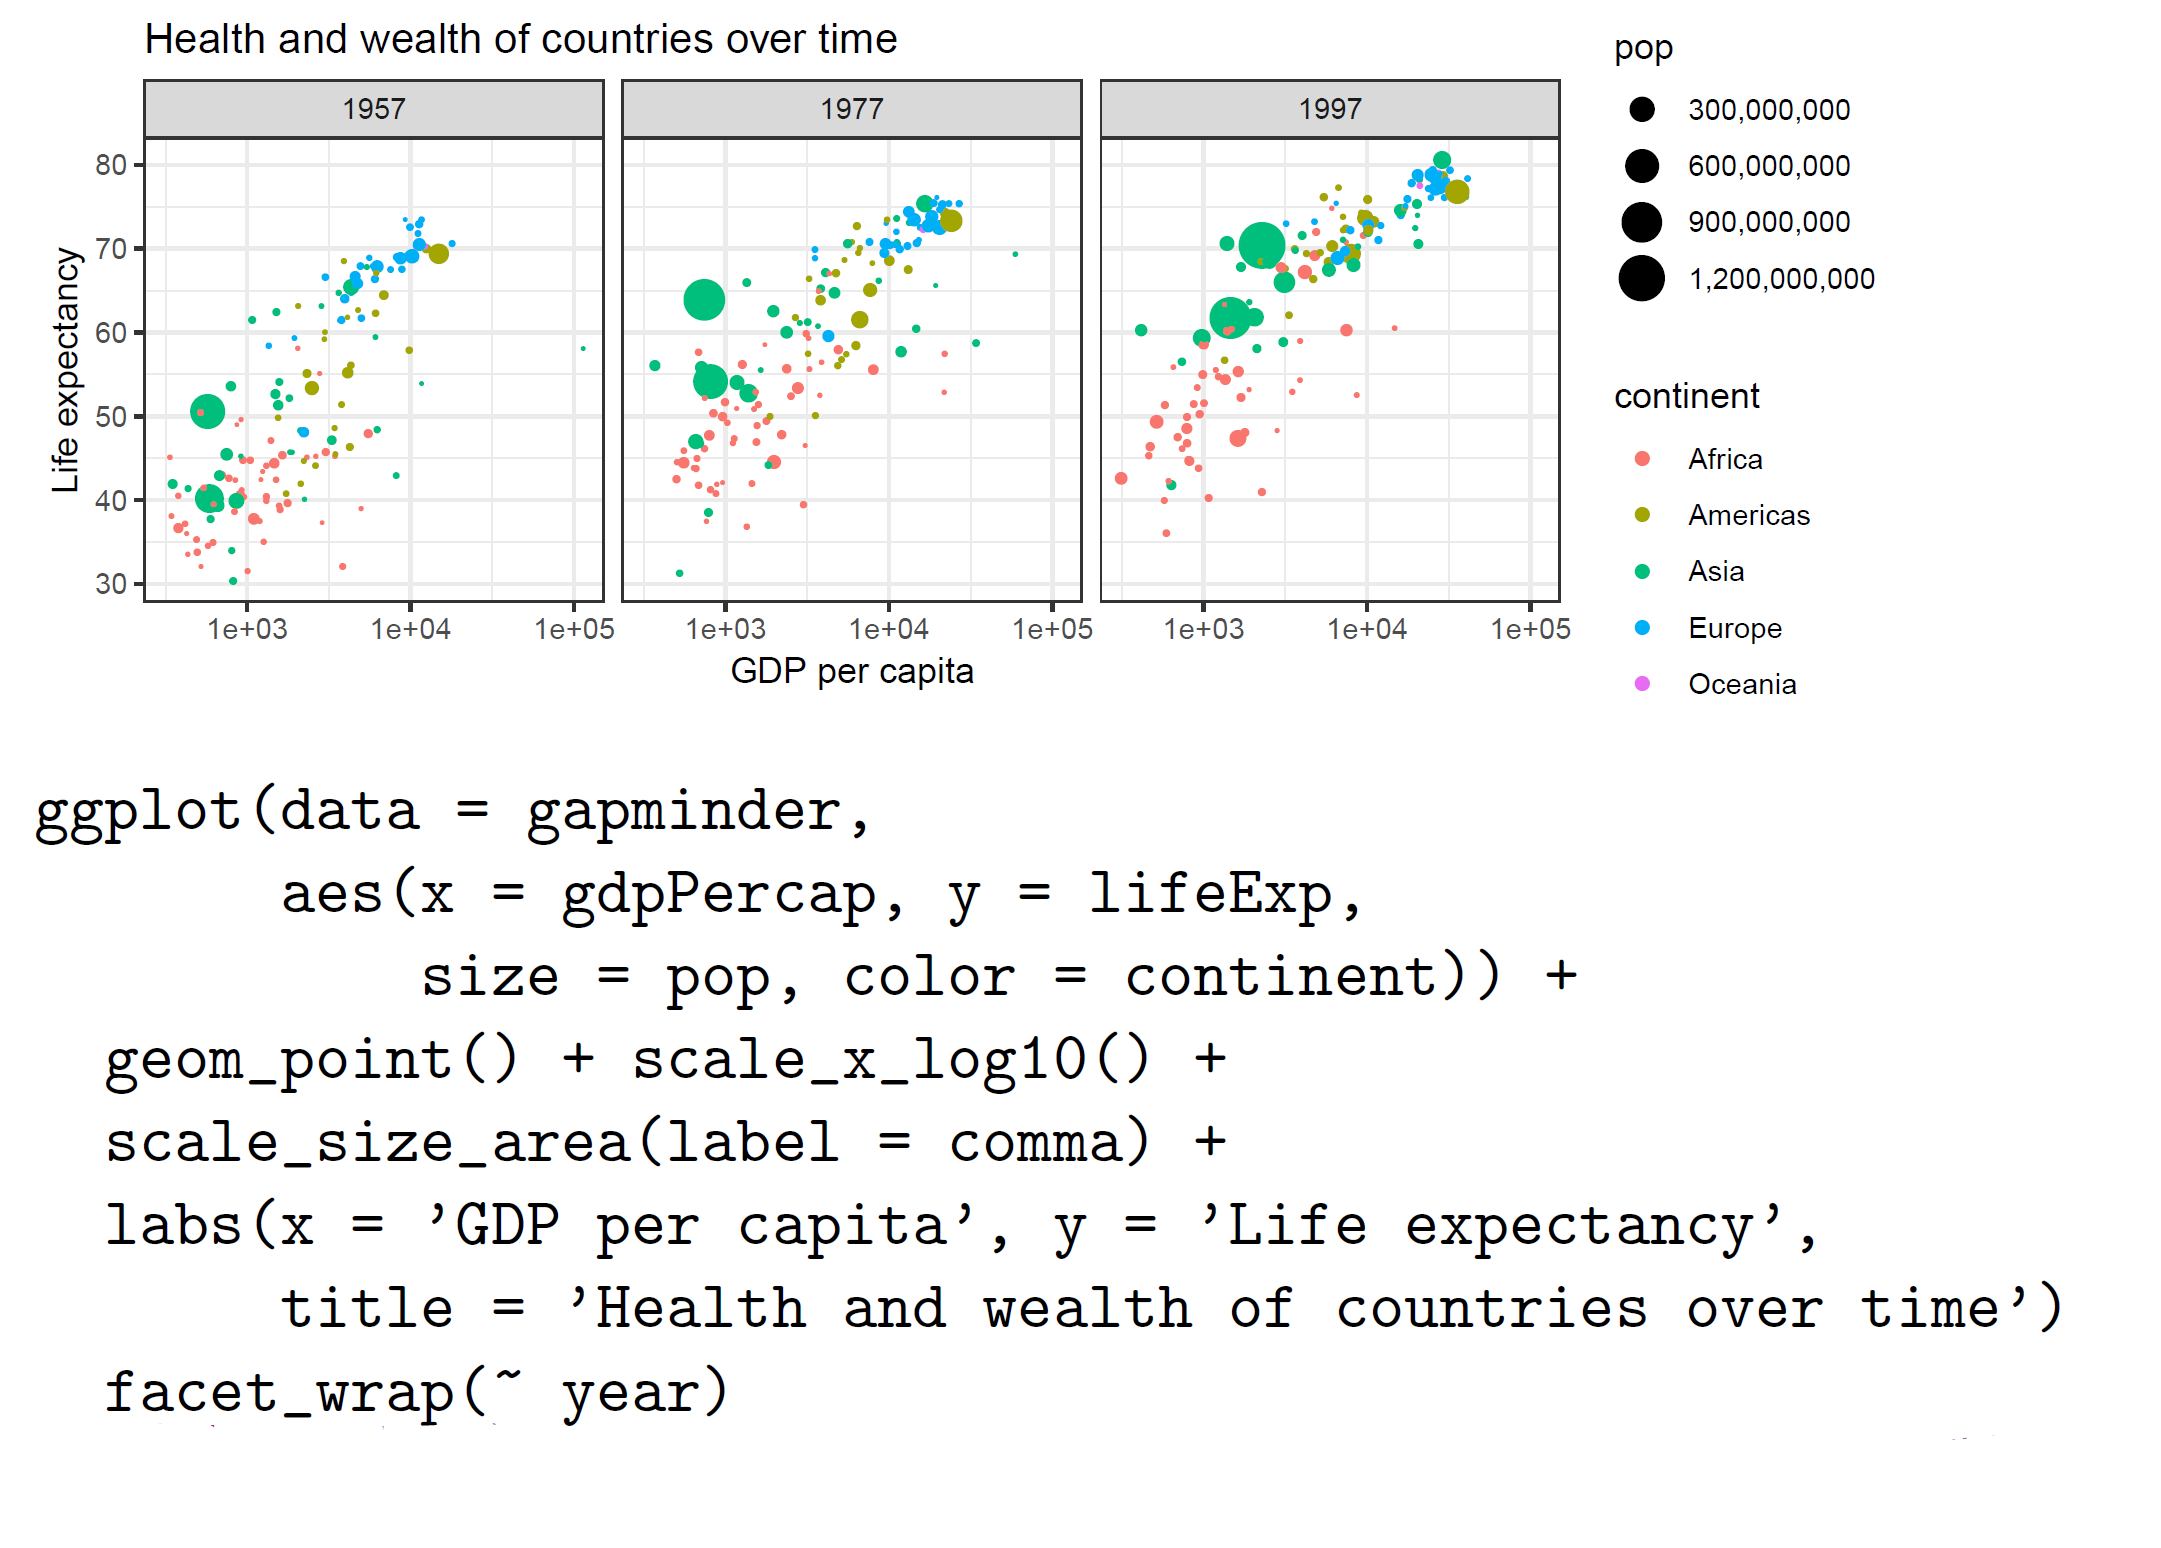
\includegraphics[width=.75\textwidth]{health_and_wealth.png}
    \caption{Plot and code necessary to build plot of the health and wealth of different countries over time.}
    \label{fig:health_and_wealth}
\end{figure}
\begin{flushleft}
If you haven't been able to understand the benefits of using ggplot and in general data visualization yet then I feel a bit bad for you, but let me recap here just in case.
\end{flushleft}
\begin{itemize}
    \item Data visualization lowers the barrier to asking questions of your data
    \item Lets you explore more, and faster
    \item Allows you to easily produces publication-ready plots
    \item Large and active user base for support
\end{itemize}



%----------------------------------------
% Step 3:
% Rename uni.tex to match your uni,
% edit the filename accordingly below,
% and put your notes in this file
%----------------------------------------

\end{document}

%%% Local Variables:
%%% mode: latex
%%% TeX-master: t
%%% End: